\vspace*{1em}

{\bf Notation.} Let $m$ be a modulus. By $\zz/m$ or $\zz/m\zz$ we mean the set of equivalence classes of integers with respect to the following (equivalence) relation
\[a \sim b \iff a \equiv b \modar{m}\]
For any $a \in \zz$, its equivalence class will be denoted as $\overline{a}$ or $[a]$.\\
\\
Essentially, $\overline{a}$ is the set that collects all integers that leave behind the same remainder as $a$ when divided by $m$, i.e. have the same natural representative modulo $m$ as $a$. Note that $\overline{a} = \overline{r}$, where $r$ is the natural representative of $a$ modulo $m$.\\
\\
\emph{e.g.}\quad $m = 2,\ a = 1$, \[\overline{1} = \set{\ldots,-3,-1,1,3,5,\ldots} = \setp{1 + 2n}{n \in \zz}\]
$m = 5,\, a = 7$, 
\[\overline{7} = \set{\ldots,-8,-3,2,7,12,17,\ldots} = \overline{2} = \setp{2 + 5n}{n \in \zz}\]
\\
Proposition \ref{modps} can be recast as saying \emph{addition and multiplication are well-defined operations on $\zz/m\zz$} (i.e., $\zz/m\zz$ is a ring).

\vspace*{2.5em}

{\bf Division of integers modulo $m$.}
\begin{itemize}
\item[(1)] With $\qq,\, \rr$ or $\cc$, we can divide by any non-zero number to solve linear equations. Consider, for example, $(2 + 3i)z = 5$; then
\begin{align*}
z= \frac{5}{2+3i}&= \frac{5}{2+3i}\cdot\frac{2 - 3i}{2 - 3i}\\[0.5em]
&= \frac{5(2 - 3i)}{(2+3i)(2 - 3i)}\\[0.5em]
&= \frac{10 - 15i}{2^2 + 3^2} = \frac{10}{13} - \frac{15}{13}i
\end{align*}
\item[(2)] With $\zz$, division can be tricky: $3x = 5$ has no integer solutions, but $3x = 6$ has $x = 2$ as a solution.
\item[(3)] When can we divide in $\zz/m\zz$?
\end{itemize}

\vspace*{2em}

\begin{definition}
Let $m$ be a modulus and $a$ an integer. Say that $b \in \zz$ is a \emph{multiplicative inverse of $a$ modulo $m$} if
\[ab \equiv 1\modar{m}\]
\emph{e.g.}\quad $m = 11$ and $a = 4$. Then $b = 2$ is \emph{not} a multiplicative inverse of $a$, since \[ab = 8 \not\equiv 1 \modar{11}.\]
But $b = 3$ is, because $ab = 12 \equiv 1 \modar{11}$.\\
\\
In fact, any other integer $c$ such that $ac \equiv 1\modar{11}$ will be of the form $3 + 11n$. 
%Since, 
%\[c \equiv 12c \equiv 3(ac) \equiv 3\modar{11}\]
\end{definition}

\vspace*{1em}

When $a$ has a multiplicative inverse $b$ modulo $m$, we can solve linear equations of the form
\[ax \equiv c \modar{m}\]
easily.\\
\\
Multiply by $b$, and you get $(ba)x \equiv bc\modar{m}$. Since $ba \equiv 1 \modar{m}$, we obtain $x \equiv (ba)x \equiv bc \modar{m}$.\\
\\
\emph{e.g.} Let's solve $4x \equiv 7\modar{11}$. We found $b = 3$ is a multiplicative inverse of $4$ modulo $11$, therefore
\[x \equiv (3\cdot 4)x \equiv 3\cdot (4x) \equiv 3\cdot 7\equiv 21 \equiv 10\modar{11}\]
So, when does a given integer have a multiplicative inverse with respect to a given modulus?

\vspace*{1.5em}

\begin{theorem}\label{modinv}
Let $m$ be a modulus and $a$ an integer. Then
\begin{itemize}
\item[(1)] $a$ has a multiplicative inverse modulo $m$ if and only if $\gcd(a,m) = 1$.
\item[(2)] When $a$ has a multiplicative inverse modulo $m$, then any two multiplicative inverses are necessarily congruent modulo $m$. That is, they define the same equivalence class in $\zz/m\zz$.
\end{itemize}
\end{theorem}
\begin{proof}\hfill
\begin{itemize}
\item[(1)] ($\Rightarrow$) Say $b$ is the multiplicative inverse of $a$ modulo $m$, that is $ab \equiv 1 \modar{m}$. So, $m\mid (ab - 1)$ and therefore $ab - 1 = mx$ for some $x\in \zz$. Hence $ab + m(-x) = 1$, and thus $\gcd(a,m)\mid 1$; so $\gcd(a,m) = 1$, necessarily.\\
\\
($\Leftarrow$) Suppose $\gcd(a,m) = 1$, then by B\'ezout's Identity there exist $x,y \in \zz$ such that $ax + my = 1$. Therefore $ax \equiv 1 \modar{m}$, and hence $x$ is a multiplicative inverse of $a$ modulo $m$.
\item[(2)] Say $b$ and $b'$ are two multiplicative inverses of $a$ modulo $m$, then
\[b = b\cdot 1\equiv b(ab')\equiv (ba)b' \equiv 1\cdot b' \equiv b'\modar{m}\]\\[-5em]
\end{itemize}
\end{proof}

\vspace*{0.5em}

\begin{example}[in-class]\hfill
\begin{itemize}
\item[(1)] Find the multiplicative inverse of $15$ modulo $37$.
\item[(2)] Using (1), solve the linear equation/congruence $15x \equiv 4\modar{37}$.
\end{itemize}
\end{example}

\vspace*{1em}

\begin{corollary}
$\overline{a}$ has a \emph{unique} multiplicative inverse $\overline{b}$ in $\zz/m\zz$ if and only if $\gcd(a,m) = 1$.
\end{corollary}

\vspace*{1em}

\begin{corollary}\label{cancel}
If $\gcd(a,m) = 1$, then for any $x,y \in \zz$,
\[ax\equiv ay\modar{m} \implies x\equiv y \modar{m}\]
\end{corollary}

\vspace*{1em}

\begin{corollary}\label{primeinv}
Let $p$ be a prime number and $a \in \zz$. Then $a$ has a multiplicative inverse modulo $p$ if and only if $p\nmid a$ if and only if $\overline{a} \neq \overline{0}$ in $\zz/p\zz$. $\zz/p\zz$ is a field!
\end{corollary}

\vspace*{2.5em}

\begin{center}
{\Large Modular Dynamics}
\end{center}

Dynamics in the simplest mathematical form (discrete time): Let $X$ be a set and $f:X \to X$ a function, what happens in this sequence $x_0,\,f(x_0),\,f(f(x_0)),\,f(f(f(x_0))),\ldots, f^n(x_0),\ldots$?\\
\\
\emph{e.g.}\quad Consider $X = \nn = \zz_+ = \set{1,2,\ldots}$, let $f:\nn \to \nn$ be defined as
\[f(n) = \begin{cases}n/2 & \text{$n$ is even}\\[0.5em] 3n+1 & \text{$n$ is odd} \end{cases}\]\\
Say $x_0 = 17$, then the sequence reads: $17,\ 52,\ 26,\ 13,\ 40,\ 20,\ 10,\ 5,\ 16,\ 8,\ 4,\ 2,\ 1,\ 4,\ 2,\ 1,\ldots$
\[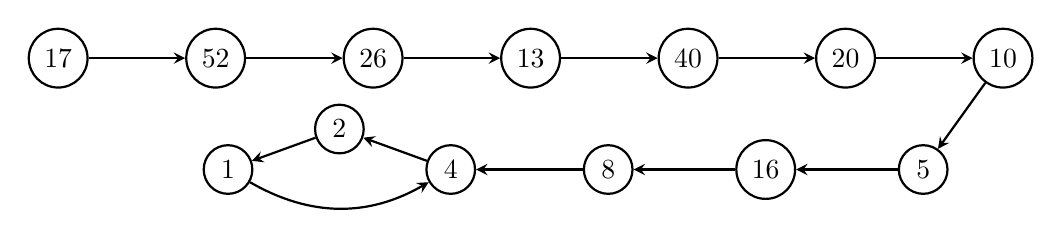
\begin{tikzpicture}[->,>=stealth,auto,node distance=2cm,
  thick,main node/.style={circle,draw}]

  \node[main node] (1) {$17$};
  \node[main node] (2) [right of=1] {$52$};
  \node[main node] (3) [right of=2] {$26$};
  \node[main node] (4) [right of=3] {$13$};
  \node[main node] (5) [right of=4] {$40$};
  \node[main node] (6) [right of=5] {$20$};
  \node[main node] (7) [right of=6] {$10$};
  \node[main node] (8) [below left of=7,xshift=0.4cm] {$5$};
  \node[main node] (9) [left of=8] {$16$};
  \node[main node] (10) [left of=9] {$8$};
  \node[main node] (11) [left of=10] {$4$};
  \node[main node] (12) [above left of=11,yshift=-0.9cm] {$2$};
  \node[main node] (13) [below left of=12,yshift=0.9cm] {$1$};
%  \node (7) [right of=6] {$\cdots$};

  \path[every node/.style={font=\sffamily\small}]
    (1) edge[] node[] {} (2)
    (2) edge[] node[] {} (3)
    (3) edge[] node[] {} (4)
    (4) edge[] node[] {} (5)
    (5) edge[] node[] {} (6)
    (6) edge[] node[] {} (7)
    (7) edge[] node[] {} (8)
    (8) edge[] node[] {} (9)
    (9) edge[] node[] {} (10)
    (10) edge[] node[] {} (11)
    (11) edge[] node[] {} (12)
    (12) edge[] node[] {} (13)
    (13) edge[bend right] node[] {} (11);
\end{tikzpicture}\]

%\vspace*{1em}

\begin{conjecture}[Collatz, $3n+1$]
For any $x_0 \in \nn$, there exists a $n>0$ such that $f^n(x_0) = 1$.
\end{conjecture}

\vspace*{2em}

{\bf Modular Dynamics.} $X = \zz/m\zz$ or some subset of $\zz/m\zz$.\\
\\
{\bf Additive Modular Dynamics.}\\[0.2em]
For a modulus $m$ and an integer $a$, we consider the dynamics of the function
\[\fbox{$+a\modar{m}$}:\zz/m\zz \to \zz/m\zz,\quad \overline{x} \mapsto \overline{x + a}\]\\
\emph{e.g.} Let $X = \zz/21\zz,\ a = 6$. We consider the dynamics of \fbox{$+6\modar{21}$} with $x_0 = 2$,
\[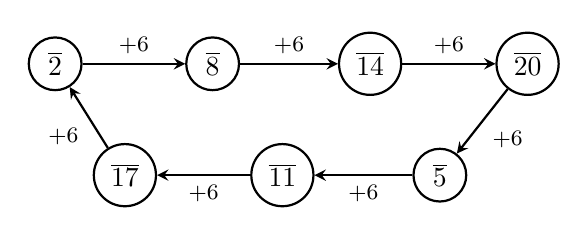
\begin{tikzpicture}[->,>=stealth,auto,node distance=2cm,
  thick,main node/.style={circle,draw}]

  \node[main node] (1) {$\overline{2}$};
  \node[main node] (2) [right of=1] {$\overline{8}$};
  \node[main node] (3) [right of=2] {$\overline{14}$};
  \node[main node] (4) [right of=3] {$\overline{20}$};
  \node[main node] (5) [below left of=4,xshift=0.3cm] {$\overline{5}$};
  \node[main node] (6) [left of=5] {$\overline{11}$};
  \node[main node] (7) [left of=6] {$\overline{17}$};

%  \path[every node/.style={font=\sffamily\small}]
%    (1) edge[bend left] node[above] {} (2)
%    (2) edge[bend left] node[above] {} (3)
%    (3) edge[bend left] node[above right] {} (4)
%    (4) edge[bend left] node[below right] {} (5)
%    (5) edge[bend left] node[below] {} (6)
%    (6) edge[bend left] node[below] {} (7)
%    (7) edge[bend left] node[left] {} (1);
\path[every node/.style={font=\sffamily\small}]
	(1) edge[] node[] {\footnotesize $+6$} (2)
	(2) edge[] node[] {\footnotesize $+6$} (3)
	(3) edge[] node[] {\footnotesize $+6$} (4)
    (4) edge[] node[] {\footnotesize $+6$} (5)
    (5) edge[] node[] {\footnotesize $+6$} (6)
    (6) edge[] node[] {\footnotesize $+6$} (7)
    (7) edge[] node[] {\footnotesize $+6$} (1);
\end{tikzpicture}\]
this is a \emph{cycle} of \emph{length} $7$.

\vspace*{1em}

\begin{proposition}
Let $m$ be a modulus and let $a$ be an integer. Then the dynamics of \fbox{$+a\modar{m}$} consists of $\gcd(a,m)$-many cycles of length $\ell = m/\gcd(a,m)$.
\end{proposition}
\begin{proof}
Suppose we start with $\overline{b} \in \zz/m\zz$
\[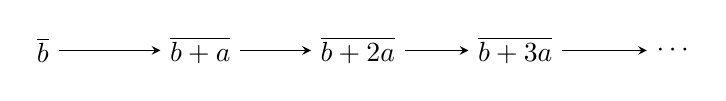
\begin{tikzpicture}[->,>=stealth,auto,node distance=2cm,main node/.style={rectangle,draw}]

  \node[] (1) {$\overline{b}$};
  \node[] (2) [right of=1] {$\overline{b+a}$};
  \node[] (3) [right of=2] {$\overline{b+2a}$};
  \node[] (4) [right of=3] {$\overline{b+3a}$};
  \node[] (5) [right of=4] {$\cdots$};

  \path[every node/.style={font=\sffamily\small}]
    (1) edge[] node[] {} (2)
    (2) edge[] node[] {} (3)
    (3) edge[] node[] {} (4)
    (4) edge[] node[] {} (5);
\end{tikzpicture}\label{cycle1}\tag{$\ast$}\]
In step $k$, we get $\overline{b + ka}$.\\
\\
Because $X = \zz/m\zz$ is a finite set, we return to $\overline{b}$ eventually (e.g. when $k = m$). Let $\ell$ be the smallest positive integer such that
\[\overline{b} = \overline{b + \ell a}\label{cycle2}\tag{$\ast\ast$}\]
and $\ell$ is necessarily the length of the cycle \refp{cycle1}.\\
\\
Rewriting \refp{cycle2}, we get $b \equiv b + \ell a\modar{m}$; equivalently, $\ell a \equiv 0 \modar{m}$. That is, $m\mid \ell a$ and $\ell$ is the smallest positive integer with this property. Therefore $\ell a = \lcm(a,m)$, and hence
\[\ell = \frac{\lcm(a,m)}{a} = \frac{m}{\gcd(a,m)}\]
So, the number of cycles $= m/\ell = \gcd(a,m)$.
\end{proof}

\vspace*{1.5em}

\begin{corollary}
If $\gcd(a,m) = 1$, then \fbox{$+a\modar{m}$} on $\zz/m\zz$ has just \emph{one} cycle of length $m$.
\end{corollary}

\vspace*{0.5in}

\subsection{Problems}
\vspace{0.1in}

\begin{problem}\label{Problem 9.1}\hfill
\begin{itemize}
\item[(1)] Find the multiplicative inverse of $15$ modulo $49$.
\item[(2)] Using (1), solve the linear equation/congruence $15x \equiv 8\modar{49}$.
\end{itemize}
\end{problem}

\vspace*{0.1in}

\begin{problem}\label{Problem 9.2}
Solve the congruences $5x \equiv 11\modar{37}$ and $11y \equiv 5\modar{37}$. If solutions exist, simplify $xy\modar{37}$.
\end{problem}

\vspace{0.1in}

\begin{problem}\label{Problem 9.3}
Consider the following modular dynamical system, which is neither additive nor multiplicative.
\begin{itemize}
\item[(a)] Let $X = \zz/13\zz$ and let $f : X \to X$ be given by
\[x \mapsto f(x) \coloneqq x^2 + 3 \modar{13}.\]
Draw the complete diagram for the dynamics of $f$.
\item[(b)] Let $A_0 = 0$ and let $A_{n+1} = f(A_n) \modar{13}$ for all integers $n \geq 0$. What is $A_{2021} \modar{13}$?
\end{itemize}
\end{problem}